\chapter{Implementing Tools with TEBNF}
This chapter focuses on the implementation of applications using TEBNF and the TEBNF code generation tool.  The chapter is divided into four sections.  The first section will showcase a real world example using a TEBNF grammar to parse data from a National Imagery Transmission Format (NITF) version 2.1 file.  The second section will walk through the implementation of two test cases.  The third section will cover the testing and verification of these test cases.  The fourth section of the chapter will cover the results of testing.

\section{NITF File Parsing: A Real World Example}
\label{sections:RealWorldNitfExample}
Software developers are oftentimes tasked to write software that parses and processes data in different formats.  A well-known example is word processing software.  Word processing software must be able to open and read documents structured in its own proprietary format and others (e.g. pdf, txt, etc.).  Creating software that reads specific data formats requires access to documentation detailing the exact structure of each format.

\indent
An example data format read by different applications is the NITF 2.1 file format.  The NITF 2.1 file format is part of a suite of standards established by the United States (US) Government for formatting digital imagery \cite{2500c_01}.  Documentation detailing the NITF 2.1 standard is freely available for download from the Geospatial Intelligence Standards Working Group’s website \cite{gwg_01}.  This file format is compatible with software used by members of the intelligence community, which includes the US Department of Defense (DoD) \cite{2500c_01}.  The VANTAGE\textsuperscript{TM} software suite produced by the Space Dynamics Laboratory and the SOCET Services suite produced by BAE Systems are all capable of reading and exploiting NITF 2.1 formatted files \cite{sdl_01,bae_01}.

\begin{figure}[htbp]
\centering
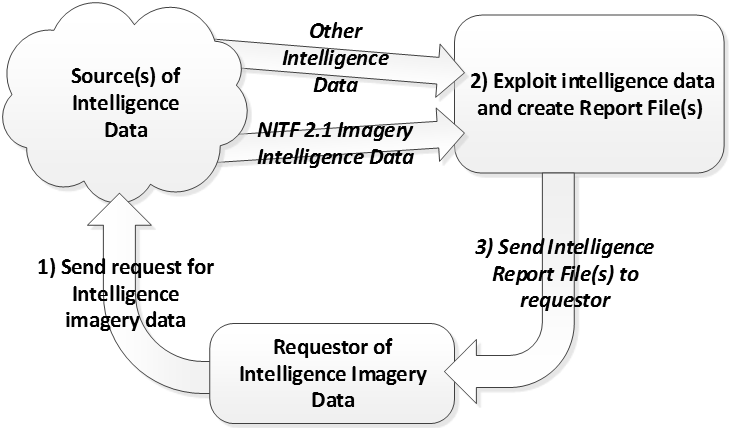
\includegraphics[width=0.9\textwidth]{figures/NitfConops.png}
\caption{Concept of operations for NITF 2.1 format files.}
\label{fig:NitfConops}
\end{figure}

\indent
As explained by \cite{2500c_01}, the stated purpose of the NITF 2.1 file format is to provide the intelligence community an interoperable means of transmission and/or storage of electronic imagery data.  The NITF 2.1 format is intended to be used in the dissemination of imagery derived intelligence data.  A general concept of operations involving NITF data is shown in figure~\ref{fig:NitfConops}.  First, imagery data in NITF 2.1 format is requested by a member of the intelligence community.  Second, the NITF data is received and combined with other collateral information to create intelligence report file(s) and/or products containing   the requested information of interest.  Third, these report files and/or products are given to the requestor of that intelligence information.

\indent
Exploiting NITF 2.1 files requires a detailed understanding of the format.  With this understanding, it is possible to create software than can parse NITF 2.1 files to find information of interest, generate report files, and/or products.

\indent
The NITF 2.1 file format is composed of a file header and one or more segments.  Each segment contains a subheader with data fields.  Each data field has a specific size and format (depending on the type of field) and is located at a specific byte offset within the file.

\indent
Conditional data and/or data characteristics can be added to NITF 2.1 files. This flexibility to extend the format is done using conditional fields in the file header and subheaders indicating the existence of Tagged Record Extensions (TREs) and Data Extension Segments.  Tagged Record Extensions contain data fields, while extension segments can contain data in new formats.

\begin{figure}[htbp]
\centering
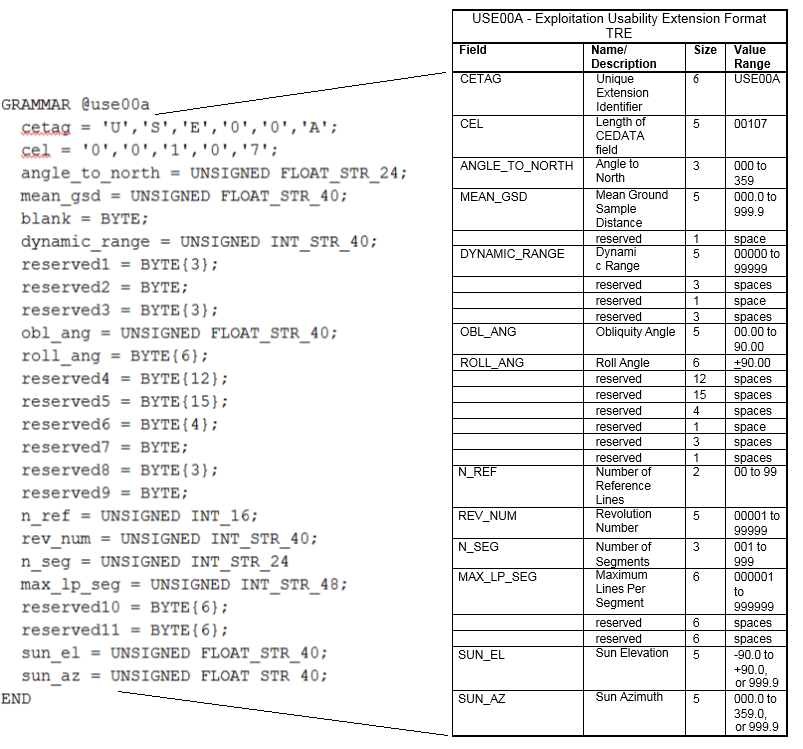
\includegraphics[width=0.9\textwidth]{figures/TreComparison.png}
\caption[TEBNF Implementation of the NITF 2.1 USE00A TRE]{TEBNF Implementation of the NITF 2.1 USE00A TRE (TRE information taken from \cite{use001_01}).}
\label{fig:tre}
\end{figure}

\indent
As stated previously, various applications such as Vantage and SOCET glean data from NITF 2.1 formatted files for exploitation (figure~\ref{fig:NitfConops}).  This can also be done using a TEBNF grammar as demonstrated in figure~\ref{fig:tre}.  The figure shows a side-by-side comparison of the NITF 2.1 USE00A (Exploitation Usability Extension Format) TRE \cite{use001_01} to its equivalent implementation in TEBNF.  Each data field for this TRE is compared to its equivalent TEBNF grammar expression.  This comparison highlights several important advantages of using TEBNF to implement parsers of specifications like NITF:
\begin{itemize}
  \item Convenience.  There is no need to keep track of the offset of each data field because it is determined based on the size of each type.
  \item Readability.  TEBNF grammar syntax looks very similar to actual specifications as shown in figure~\ref{fig:tre}, making it is easier to understand.
  \item Self-documenting.  Since TEBNF grammar syntax ties the size of each data field to the size of the subelement type, the grammar helps to document itself. 
\end{itemize}

\section{Test Cases}
In order to verify the functionality of the TEBNF language, two case studies were implemented.  Both case studies showcase the strengths of TEBNF and the TEBNF code generation tool.  Further case studies are possible because TEBNF is Turing complete (see appendix~\ref{appendix:TEBNFTuringCompletenessProof}).

\subsection{Basic Calculator}
The first test case was to create a basic calculator console application that supports addition, subtraction, multiplication, and division of integers.  Producing this calculator required the tool to generate code that:
\begin{enumerate}
  \item Parses numeric data received over a console input.
  \item Makes calculations based on the data received from that console input.
  \item Sends the results of those calculations to console output.
  \item Allows the user to exit when finished.
\end{enumerate}

\indent
The calculator begins with a step executed once at the beginning of the program. This initial step prompts users to enter a number, which is then saved as an initial “result” value because all subsequent math operations are executed against it.  From this point onward, the calculator repeats a cycle that 1) asks for a number, 2) asks for a math operator, 3) applies that math operator against the saved result and the last number entered, 4) saves the result, and 5) displays that result.   This cycle then repeats until the user enters a ‘=’ operator, which then displays the result and exits the program.

\indent
Input for the calculator is achieved with a single TEBNF console input element containing two prompt values.  The first is used for prompting the user to enter a number, accepting a signed 64-bit integer.  The second one is used for prompting the user to enter a single character (math operator).  Outputting the result of math operations is accomplished with a single TEBNF console output element.

\indent
Acceptable input values for the calculator are limited to integers or one of five math operator characters (‘+’, ‘-‘, ‘*’, ‘/’, ‘=’).  TEBNF grammar elements are defined for each math operator.  Another grammar element was created to represent a signed 64-bit integer, providing a place to store integers as they are unmarshaled from input.  The saved result value is represented as a static variable within the number grammar element, serving as a place to store the result of each math operation.  An actions element was created for each of the supported math operators.  Each actions element adds, subtracts, multiplies, divides, or sets the saved result using the last unmarshaled integer.

\begin{figure}[htbp]
\centering
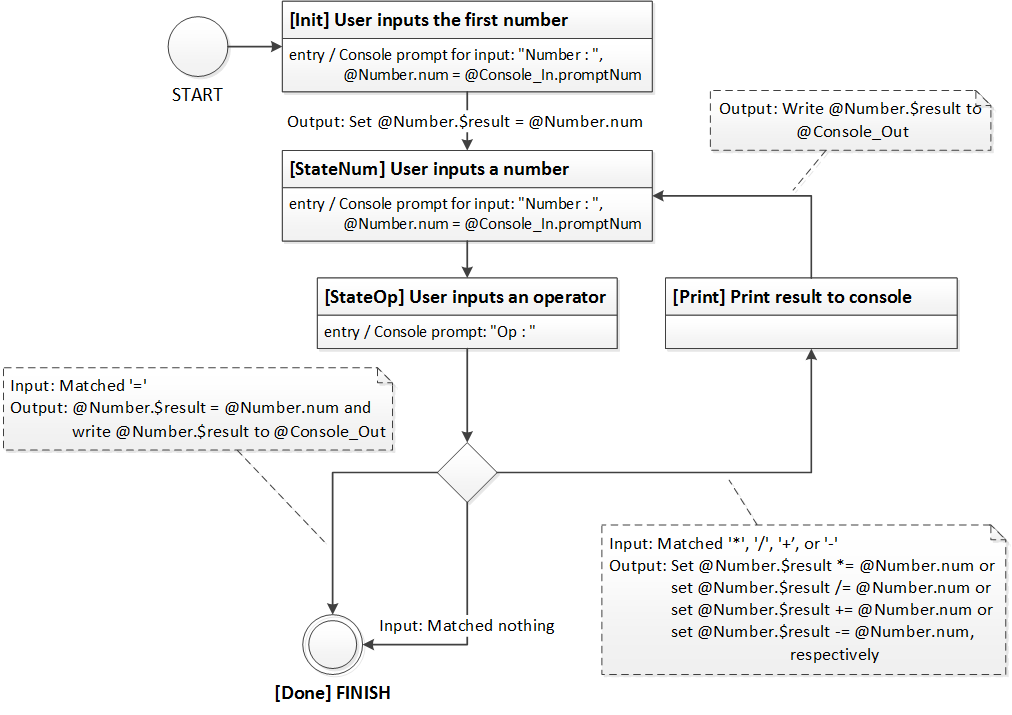
\includegraphics[width=0.9\textwidth]{figures/CalculatorUmlStateMachine.png}
\caption[State machine representing a calculator.]{State machine representing a calculator (includes pseudocode).}
\label{fig:CalculatorUmlStateMachine}
\end{figure}

\indent
The last TEBNF element included in the grammar describes the calculator as a state machine utilizing the elements described above to define the execution path of the calculator.  The TEBNF grammar that implements this calculator is provided in listing~\ref{ExampleCalculator}.

\indent
The calculator state machine is represented with five states, as shown in figure~\ref{fig:CalculatorUmlStateMachine}.  The first state of the machine is a special case entered only once at the beginning of execution.  This initial state is a necessary special case that sets the ongoing result value for subsequent math operations.  In this state the user is prompted to enter the initial number via the console input element.  The number grammar element unmarshals this input value as a signed 64-bit integer and retains a copy for later use.  The state table then executes an actions element.  This actions element sets the result static variable equal to the unmarshaled value while the machine transitions to the next state.

\indent
After setting the result value while transitioning to the first state of the main cycle, the machine uses the console input element to prompt the user to enter a number again.  This number is also unmarshaled from input and stored as before.  The state machine then transitions to the next state.

\indent
This state uses the console input element to prompt the user to enter one of the supported math operators.  The state machine does this by moving through a series of “else-if” states.  Each state uses one of the math operator grammar elements to check the same console input for a match to one of the supported math operations.  A match occurs when a grammar successfully unmarshals the input value.  Upon matching an operator the machine transitions to the print state and executes an actions element applying that operator to the result and unmarshaled number, then assigns it to the result.  As the print state transitions to the first state of the main cycle, an actions element is executed that writes the result to the console.  The cycle then continues to repeat until the user enters a '=' to exit.  Otherwise, if a '=' operator was matched, the result is written to the console as the state machine transitions to the done state.  If the input matched nothing, the state machine transitions to the done state.

\begin{table}[h]
\begin{center}
\caption{Sample input and output data for the calculator.}
\label{sampleCalculatorIoData}
\begin{tabular}{|l|l|l|} \hline
\textbf{Operand} & \textbf{Operator} & \textbf{Result} \\
\hline \hline
5	& \cellcolor{gray!25} & \cellcolor{gray!25} \\ \hline
10	& +	& 15    \\ \hline
95	& -	& -80   \\ \hline
110	& +	& 30    \\ \hline
10	& /	& 3     \\ \hline
111	& *	& 333   \\ \hline
33	& -	& 300   \\ \hline
20	& /	& 15    \\ \hline
5	& *	& 75    \\ \hline
0   & = & 75    \\
\hline                                  
\end{tabular}
\end{center}
\end{table}

\indent
Suppose this calculator is run using the sample data in table~\ref{sampleCalculatorIoData}.  The first line in the table is the initial value 5.  The second operand entered by the user is the number 10.  The '+' operator is entered by the user, and the result displayed is 15.  Entering the next value of 95 followed by the operator '-' displays the number -80.  This cycle continues until the user enters the '='  operator.

\subsection{NITF 2.1 UDP/IP File Transfer Client}
The second test case is a file transfer client that receives NITF 2.1 files over UDP/IP upon requesting them from a file server.  The server tells the client when it is done sending files so the client knows when to exit.  This requires the tool to generate code for a file client that:
\begin{enumerate}
  \item Asks the server to send it a file by sending it a message over a UDP/IP output.
  \item Receives the NITF 2.1 file from the server over a UDP/IP input.
  \item Uses the file length data field in the NITF 2.1 file to determine that it has received the entire file from the server as it was sent over UDP/IP.
  \item Writes that file to disk using a file output.
  \item Quits upon receiving a message from the server that says it is done sending files.
\end{enumerate}

\indent
The NITF 2.1 file transfer client starts by prompting the user to enter the IP address and port that will be used for sending and receiving data over UDP/IP.  After entering this information, the client immediately sends the message "“send”" to the server to request that it send a file.  Once the server receives the "“send"” message from the client, it reads a NITF 2.1 file from disk and begins sending it to the client over UDP/IP.  As the client receives data from the server, it continually checks to see if it has received the entire NITF 2.1 file from the server.  The client knows a file transfer is complete when it has received the amount of data specified in the NITF file’s file length data field.  The client then prompts the user to enter a path including the file name specifying where the file will be written to disk.  After writing the file to disk, the client requests the next file from the server.

\indent
Allowed input values for the client are limited to a string for the IP address, an unsigned integer for the port, and strings for file paths.  All other input to the client comes from the server through a TEBNF UDP/IP input element.  A UDP/IP output element is used by the client to send data to the server.  One file output element is used by the client for writing files to disk received from the server.

\indent
A grammar element was created to find NITF 2.1 files in data received over UDP/IP.  The beginning of each NITF 2.1 file can be found by searching for the byte sequence "NITF02.10", which is always found at the beginning of each file.  The NITF 2.1 file header has a data field containing the length of the file.  This is leveraged by the TEBNF grammar element to calculate the end offset of each file.   A second grammar element was created for finding the "“done”" message in incoming data.  A third grammar was created to define the send message.  The TEBNF grammar that implements this file transfer client is provided in listing~\ref{ExampleUDPNitfReceiver}.

\begin{figure}[htbp]
\centering
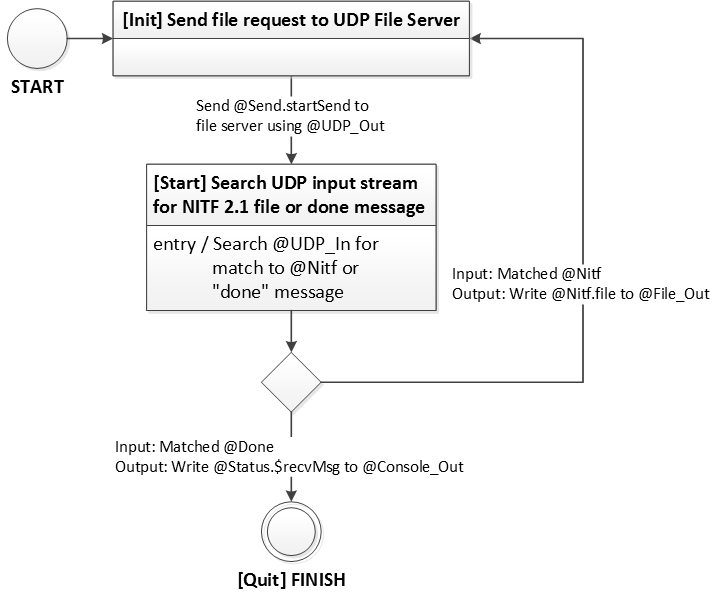
\includegraphics[width=0.9\textwidth]{figures/NitfFileClientUmlStateMachine.png}
\caption[State machine representing a NITF 2.1 UDP/IP file transfer client]{State machine representing a NITF 2.1 UDP/IP file transfer client (includes pseudocode).}
\label{fig:NitfFileClientUmlStateMachine}
\end{figure}

\indent
The file transfer client can be represented as a state machine with three states, as shown in figure~\ref{fig:NitfFileClientUmlStateMachine}.  While transitioning from the first state to the second, the “send” message is sent via the UDP/IP output element to the file server.

\indent
The second state looks at data received from the file server over the UDP/IP input element to determine if it contains a NITF 2.1 file or the "“done”" message.  If the incoming data contains a NITF file, the state machine writes it to the file output element while transitioning to the back to the first state which tells the server to send the next file, which prompts the user for a path to write the file to.  The state machine then transitions back to the first state which tells the server to send the next file.  If the incoming data does not contain a file, an "“else-if”" case in this same state checks for the “done” message.  If the done message was received, the machine writes a message to the console output telling the user that all files have been received, after which the machine transitions to the quit state and exits.

\indent
In a hypothetical case, assume there are five NITF 2.1 files to be sent to a test case file client.  Each file has a specific file size, as shown in table~\ref{sampleNitfSizeServerData}.

\begin{table}[h]
\begin{center}
\caption{Sizes of sample NITF 2.1 files sent to the test client.}
\label{sampleNitfSizeServerData}
\begin{tabular}{|c|} \hline
\textbf{NITF 2.1 File Size (bytes)} \\ \hline \hline
828710 \\ \hline
4021118 \\ \hline
912294 \\ \hline
3516054 \\ \hline
998822 \\ \hline                                  
\end{tabular}
\end{center}
\end{table}

\indent
The NITF 2.1 file server would be started and begin listening on its UDP/IP socket for the "send" request from a client.  The test case file client is then started and immediately sends a "send" request to the server, and a file transfer begins.  The UDP server reports the size in bytes of each file sent.  The file client writes each file to local disk.  The size in bytes of each file received corresponds to the size the files sent by the server.

\section{Results}
C++ code was successfully generated by the TEBNF code generation tool for each of the test cases.  The TEBNF code generation tool provides useful output when it generates code from a supplied input grammar.  The tool displays information  indicating when each stage of the code generation process finishes.  Status for the generation stage displays the classes generated for each element.  After the  generation stage finishes and all of the code has been generated, the tool reports success and the number of element files generated.  Console output from generating code for the calculator test case and the NITF 2.1 file client test case is shown in figures~\ref{fig:TestCaseBuildCalculator} and ~\ref{fig:TestCaseBuildNitfReceiver}.

\begin{figure}[h!]
\centering
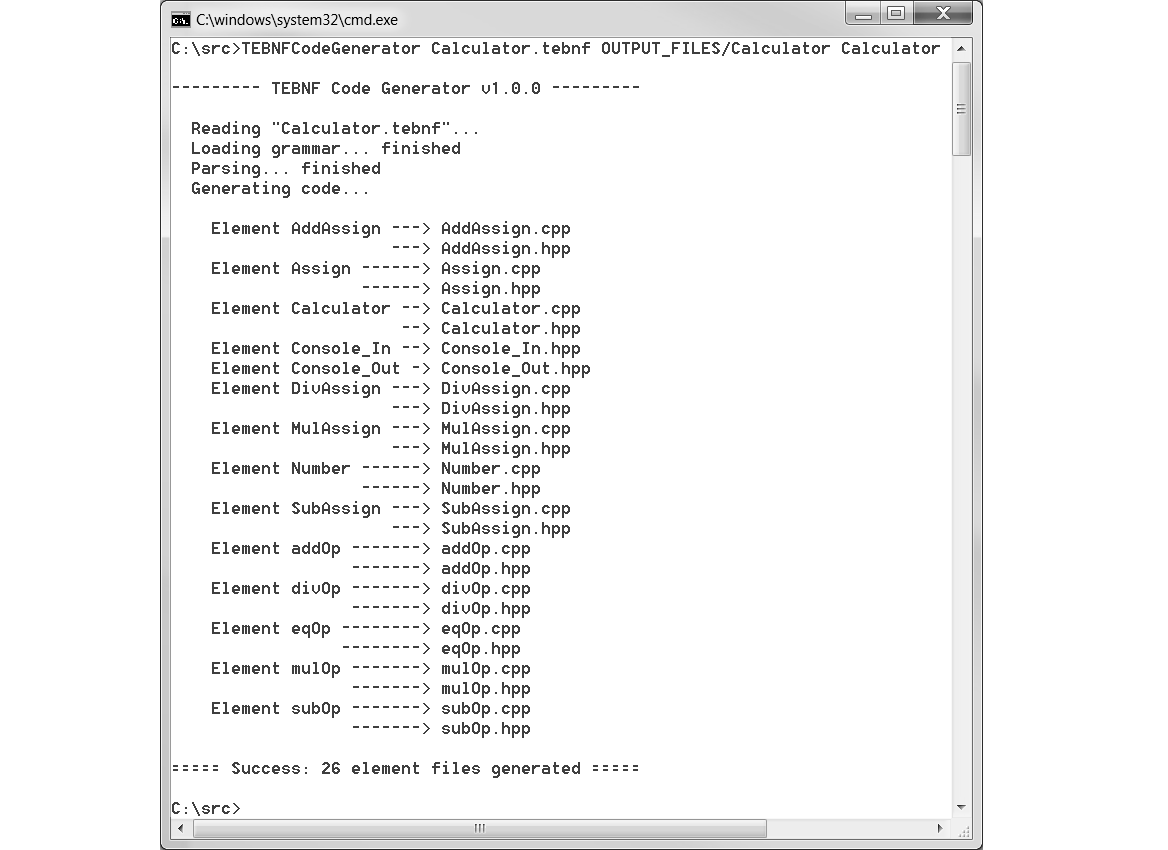
\includegraphics[width=0.9\textwidth]{figures/TestCaseBuildCalculator.png}
\caption{TEBNF code generation tool output for the calculator test case.}
\label{fig:TestCaseBuildCalculator}
\end{figure}

\begin{figure}[h!]
\centering
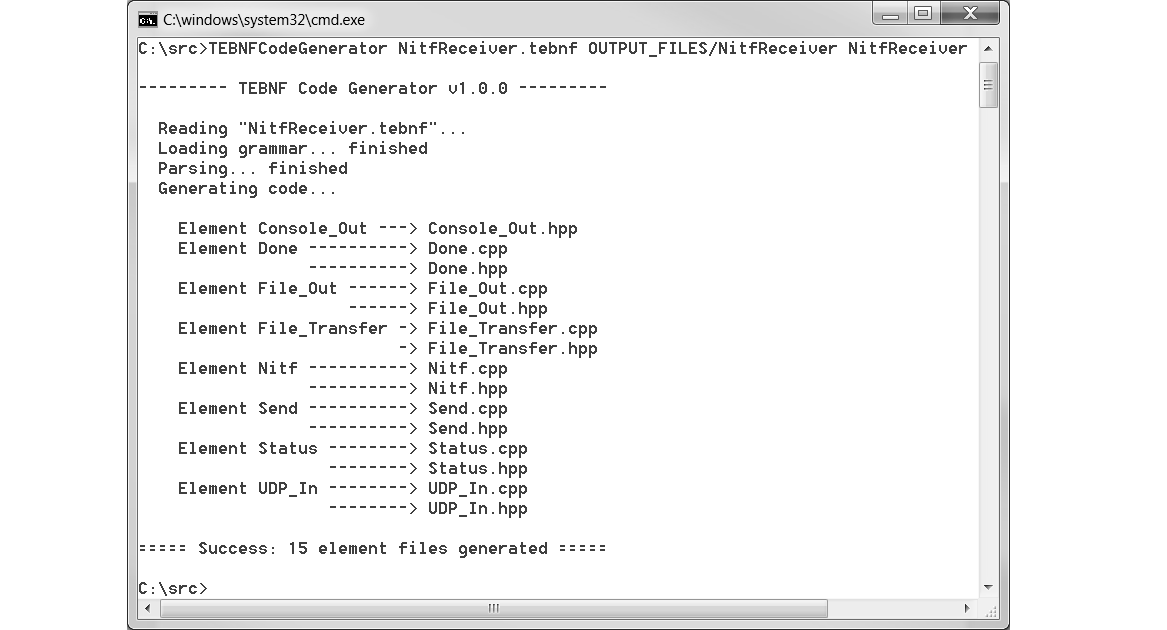
\includegraphics[width=0.9\textwidth]{figures/TestCaseBuildNitfReceiver.png}
\caption{TEBNF code generation tool output for the UDP NITF 2.1 file client test case.}
\label{fig:TestCaseBuildNitfReceiver}
\end{figure}

\indent
A CMakeLists.txt file was correctly generated by the TEBNF code generation tool for each test case, and CMake version 3.0.2 was run using those CMakeLists files to generate Microsoft Visual Studio 2013 solution and project files.  The project files generated by CMake for both test cases were successfully opened and built in Microsoft Visual Studio 2013.

\subsection{Calculator}
\label{subsections:GeneratedCalculator}
The calculator test case executable was run using the test data from table~\ref{sampleCalculatorIoData}.  As expected, the input and output of the calculator (figure~\ref{fig:TestCaseRunCalculator}) matched what is defined in table~\ref{sampleCalculatorIoData}.  This means the behavior of the calculator test case matches the behavior defined in the TEBNF grammar it was generated from.

\begin{figure}[h!]
\centering
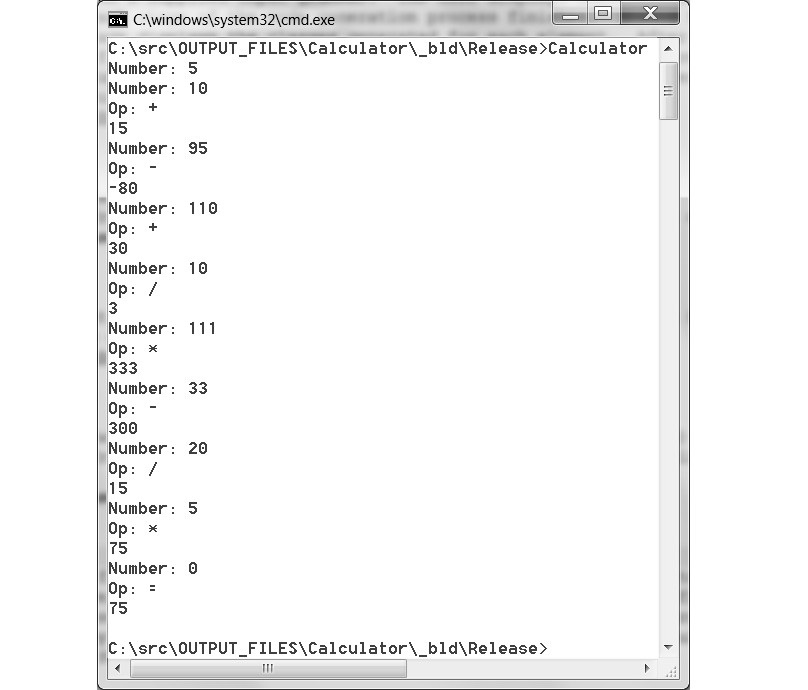
\includegraphics[width=0.9\textwidth]{figures/TestCaseRunCalculator.png}
\caption{Running the calculator test case.}
\label{fig:TestCaseRunCalculator}
\end{figure}

\subsection{NITF 2.1 File Client}
\label{subsections:GeneratedFileClient}
The NITF 2.1 file client test case executable was run using the five sample NITF 2.1 files whose sizes are found in table~\ref{sampleNitfSizeServerData}.  A NITF 2.1 file server was created that listened for client "send" requests over a UDP/IP socket on localhost port 10042.  This server was started, then the test case client was started and configured to send requests and receive file transfers on localhost port 10042.  The expected outcome occurred, with the server successfully sending five files as indicated by the first five send messages output by the server in figure~\ref{fig:TestCaseRunNitfServer}.  This was followed by the last four byte "done" message is sent to notify the client it was done sending.  The same five files were received by the client which prompted for a file name to save each file as shown in  figure~\ref{fig:TestCaseRunNitfReceiver}.  After saving the files, the client exited because the server had sent the "done" message.

\begin{figure}[h!]
\centering
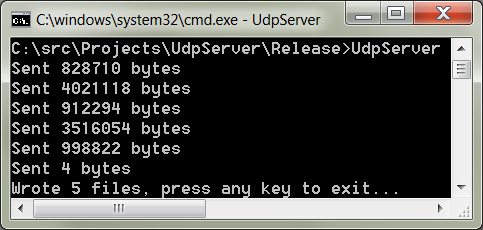
\includegraphics[width=0.9\textwidth]{figures/TestCaseRunNitfServer.png}
\caption{Running the file server for the NITF 2.1 file client test case.}
\label{fig:TestCaseRunNitfServer}
\end{figure}

\begin{figure}[h!]
\centering
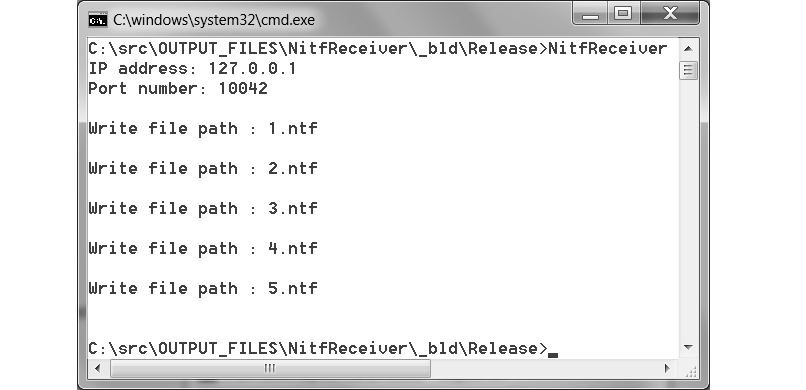
\includegraphics[width=0.9\textwidth]{figures/TestCaseRunNitfReceiver.png}
\caption{Running the NITF 2.1 file client test case.}
\label{fig:TestCaseRunNitfReceiver}
\end{figure}

\indent
The sizes of the files received were an exact match to the file sizes listed in table~\ref{sampleNitfSizeServerData}, as the output of the server and client test case executables show in figures~\ref{fig:TestCaseRunNitfServer} and~\ref{fig:TestCaseRunNitfReceiver}, respectively.  This verifies that the behavior of the NITF 2.1 client test case matches the behavior defined in the TEBNF grammar it was generated from.

\section{Comparing C++ to TEBNF}
\label{sections:ComparingCplusplusToTEBNF}
A non-generated C++ implementation of each test case was also written.  The state machines described in chapter~\ref{chapters:Design} for both test cases served as the starting point of each implementation.  Using the same design as the generated test cases, a baseline was established for more direct comparisons.

\subsection{Test Case Experience}
The non-generated C++ implementation of both test cases was verified by following the procedures outlined in subsections~\ref{subsections:GeneratedCalculator} and~\ref{subsections:GeneratedFileClient}.  Each was verified to have the same behavior and output as the test cases generated from TEBNF.

\indent
The TEBNF grammar for each test case was significantly shorter than its manual C++ counterpart.  The non-generated C++ implementations had fewer lines of code than their counterparts generated from TEBNF.  These results were expected because the TEBNF code generation tool does not yet perform optimization.

\indent
Writing code to handle I/O and input verification took longer in C++ than TEBNF, which only requires a declaration to setup any of the supported I/O methods.  Though this inconvenience was observed while writing the calculator test case in C++, it was far more noticeable while writing the client.  The client uses three different I/O methods whereas the calculator only uses one.  It is evident that a more complicated application can be more convenient to write in TEBNF than C++.  The time it took to implement both test cases in C++ and TEBNF are listed in tables~\ref{calcImplementationTimes} and~\ref{testCaseNitfRecvTimes}.

\begin{table}[h]
\begin{center}
\caption[Calculator Test Case Implementation Times]{Calculator Test Case Implementation Times (measured in hours).}
\label{calcImplementationTimes}
\begin{tabular}{|c|c|c|} \hline
\textbf{Item to Implement} & \textbf{C++} & \textbf{TEBNF} \\ \hline \hline
Console I/O                & 1            & 0.1            \\ \hline
State Machine              & 1            & 0.5            \\ \hline
\textbf{Total}             & \textbf{2}   & \textbf{0.6}   \\ \hline
\end{tabular}
\end{center}
\end{table}

\begin{table}[h]
\begin{center}
\caption[NITF File Client Test Case Implementation Times]{NITF File Client Test Case Implementation Times (measured in hours).}
\label{testCaseNitfRecvTimes}
\begin{tabular}{|c|c|c|} \hline
\textbf{Item to Implement} & \textbf{C++} & \textbf{TEBNF} \\ \hline \hline
Console I/O                & 1            & 0.1            \\ \hline
File I/O                   & 1            & 0.1            \\ \hline
UDP/IP I/O                 & 4            & 0.5            \\ \hline
State Machine              & 4            & 1              \\ \hline
\textbf{Total}             & \textbf{10}  & \textbf{1.7}   \\ \hline
\end{tabular}
\end{center}
\end{table}

\indent
Another disparity in coding effort was observed while writing the NITF file parser in C++.  Creating NITF parsing code in C++ took a lot more effort than in TEBNF.  The non-generated implementation required calculation of an offset whenever it was necessary to jump to a specific location in the NITF file.  Calculation of this offset requires knowledge beforehand of the size and position of each field.  On top of this, fields in the NITF standard can vary in length and be of different formats, as explained in section~\ref{sections:RealWorldNitfExample}.  Compare this effort to the TEBNF implementation found in listing~\ref{ExampleUDPNitfReceiver} which made it possible to write a parser resembling the actual specification document itself.

\subsection{Test Case Analysis}
A widely accepted metric for measuring code complexity is McCabe's Cyclomatic Complexity \cite{cardoso_01}.  This metric was derived from graph theory by McCabe to measure the number of control flow paths in a code module \cite{cardoso_01}.  McCabe's Cyclomatic Complexity is $ e - n + 2 $, where $e$ is the number edges in the control flow graph and $n$ is the number of nodes \cite{cardoso_01}.  An example of its use proposed by \cite{zhang_01} employs McCabe's Cyclomatic Complexity metric to effectively predict defects in code modules.

\indent
The Lizard code complexity analyzer \cite{lizard_01} tool was used to analyze each test case.  The analysis results from the tool contained several valuable metrics, including the average cyclomatic complexity number (CCN) \cite{lizard_01} of every function in the test cases.  The analysis results of each test case are provided in tables~\ref{LizardAnalysisFileClient} and \ref{LizardAnalysisCalculator}.  Values related to the interquartile range (IQR) were calculated from the analysis data of each test case, including the lower (first) quartile (Q1) corresponding to the $25^{th}$ percentile, the higher quartile (Q3) corresponding to the $75^{th}$ percentile, and the median.  In order to focus on the most relevant analysis data, the upper limit ($U_{CCN}$) and lower limit ($L_{CCN}$) of each data set was calculated as $Q3 + 1.5(IQR)$ and $Q1 - 1.5(IQR)$, respectively.

\begin{table}[h]
\begin{center}
\caption{Analysis results for the NITF file client test cases.}
\label{LizardAnalysisFileClient}
\begin{tabular}{|l|c|c|c|c|} \hline
\textbf{Test Case} & \textbf{Avg. CCN} & $\mathbf{U_{CCN}}$ & \textbf{Avg. Token Count} & \textbf{Func. Count} \\ \hline \hline
Generated     & 2.00 & 3 & 54.49  & 136 \\ \hline
Non-generated & 3.38 & 6 & 101.81 & 16  \\ \hline
\end{tabular}
\end{center}
\end{table}

\begin{table}[h]
\begin{center}
\caption{Analysis results for the calculator test cases.}
\label{LizardAnalysisCalculator}
\begin{tabular}{|l|c|c|c|c|} \hline
\textbf{Test Case} & \textbf{Avg. CCN} & $\mathbf{U_{CCN}}$ & \textbf{Avg. Token Count} & \textbf{Func. Count} \\ \hline \hline
Generated     & 1.89 & 3 & 49.50 & 135 \\ \hline
Non-generated & 3.42 & 7 & 81.42 & 12  \\ \hline
\end{tabular}
\end{center}
\end{table}

\indent
The data in tables~\ref{LizardAnalysisFileClient} and \ref{LizardAnalysisCalculator} show differences between the generated and non-generated test cases.  Compared to the non-generated C++ implementations, the test cases generated from TEBNF have (1) more functions, (2) a lower average number of tokens per function, and (3) a lower average CCN per function.

\begin{table}[h]
\begin{center}
\caption{P-values calculated from the analysis data of each test case.}
\label{LizardAnalysisPvalues}
\begin{tabular}{|l|c|c|} \hline
\textbf{Test Case} & $\mathbf{P_{CCN}}$ & $\mathbf{P_{TokenCount}}$ \\ \hline \hline
File Client & 0.041236 & 0.007916 \\ \hline
Calculator  & 0.017212 & 0.043956 \\ \hline
\end{tabular}
\end{center}
\end{table}

\indent
Tables~\ref{LizardAnalysisFileClient} and \ref{LizardAnalysisCalculator} illustrate the similarity in CCN values measured by the analysis tool for generated and non-generated code.  According to \cite{linuxJournal_01}, CCN values $\leq$ 10 fit inside the low risk category.  Given that (1) the non-generated test cases were built specifically to mimic the behavior of the generated test cases, (2) the average CCN values for all of the test cases fall into the low risk category, and (3) are close to one another in value, it can be concluded that the non-generated test cases are comparable to their generated counterparts.

\indent
Analysis data for the generated and non-generated test cases also show that they are provably different despite their similarities.  Table~\ref{LizardAnalysisPvalues} contains the p-values calculated from the data sets of each test case.  All of the p-values are significant at p $<$ 0.05, supporting the conclusion that the data sets (the test cases) are different from one another.

\begin{figure}[h!]
\centering
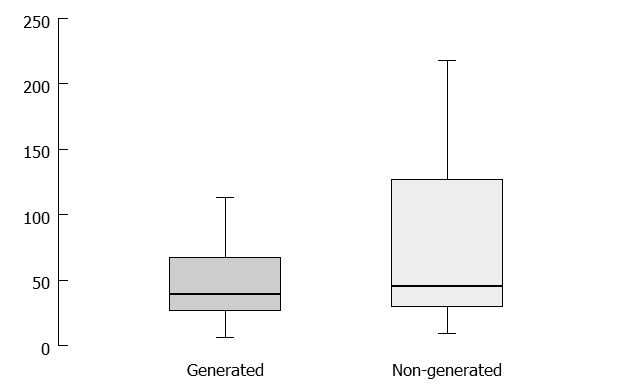
\includegraphics[width=0.9\textwidth]{figures/Lizard_FileClient_TokenCount.png}
\caption[Function token count for the file client test cases.]{Function token count for the file client test cases (omits outliers).}
\label{fig:Lizard_FileClient_TokenCount}
\end{figure}

\begin{figure}[h!]
\centering
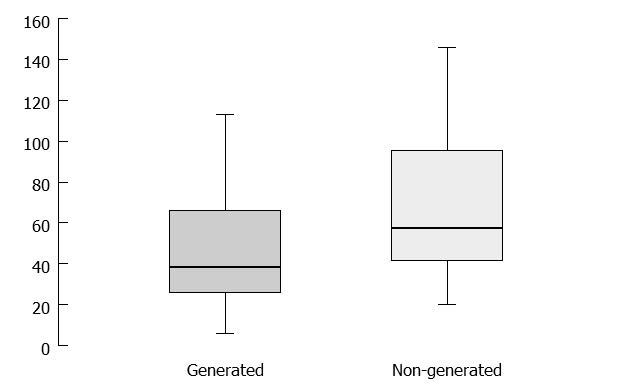
\includegraphics[width=0.9\textwidth]{figures/Lizard_Calculator_TokenCount.png}
\caption[Function token count for the calculator test cases.]{Function token count for the calculator test cases (omits outliers).}
\label{fig:Lizard_Calculator_TokenCount}
\end{figure}

\indent
Tables~\ref{LizardAnalysisFileClient} and \ref{LizardAnalysisCalculator} show that the generated code has a lower average token count per function than the non-generated code (figures~\ref{fig:Lizard_FileClient_TokenCount} and \ref{fig:Lizard_Calculator_TokenCount}).  The first conclusion to be drawn from the data as plotted in these figures is that the generated code is splitting larger computational problems into smaller tasks.  This conclusion can be drawn based on the fact that lower median values within smaller data spreads point to a greater number of functions with lower token counts.

\indent
The lower average CCN for generated code (tables~\ref{LizardAnalysisFileClient} and \ref{LizardAnalysisCalculator}) is the strongest indicator that larger computational problems are being broken down into smaller ones.  Figures~\ref{fig:Lizard_FileClient_CCN} and \ref{fig:Lizard_Calculator_CCN} show that the median CCN for the generated test cases are at or below the lowest values measured for the non-generated test cases.  Given that \cite{zhang_01} was able to use CCN values to detect the presence of defects in code, and that the generated code has shorter interquartile ranges paired with medians at or below the lowest quartiles of the non-generated code, it can be concluded that a greater number of functions in the code generated from TEBNF have a lower number of defects than the non-generated code.  This correlation of fewer defects per function in generated code means it is likely that as applications increase in size and scope, the number of defects will remain lower than application code not generated from TEBNF.

\indent
More than one participant is needed in order to conduct tests that are statistically significant.  Nevertheless, the trends observed in the analysis are interesting and worthy of future investigation.

\begin{figure}[h!]
\centering
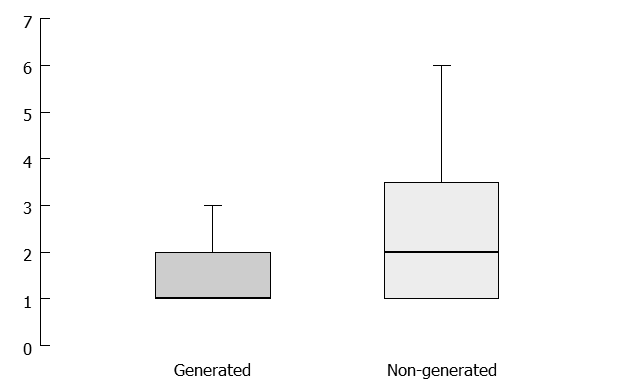
\includegraphics[width=0.9\textwidth]{figures/Lizard_FileClient_CCN.png}
\caption[Function CCN for the file client test cases.]{Function CCN for the file client test cases (omits outliers).}
\label{fig:Lizard_FileClient_CCN}
\end{figure}

\begin{figure}[h!]
\centering
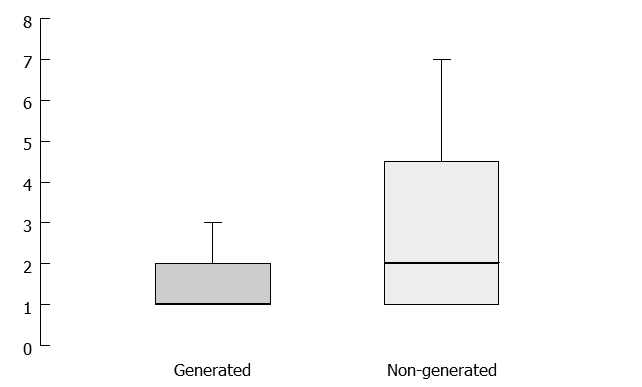
\includegraphics[width=0.9\textwidth]{figures/Lizard_Calculator_CCN.png}
\caption[Function CCN for the calculator test cases.]{Function CCN for the calculator test cases (omits outliers).}
\label{fig:Lizard_Calculator_CCN}
\end{figure}






